\documentclass[aspectratio=169]{beamer}



% OPCIONES DE BEAMER

\definecolor{Maroon}{cmyk}{0, 0.87, 0.88, 0.1}
\definecolor{teal}{rgb}{0.0, 0.45, 0.45}

\usetheme[block=fill, subsectionpage=progressbar, titleformat section=smallcaps]{metropolis}
\setbeamertemplate{frametitle continuation}[roman]
\setbeamertemplate{section in toc}[balls numbered]
\setbeamertemplate{subsection in toc}[subsections unnumbered]
%\setsansfont[BviejoFont={Fira Sans SemiBold}]{Fira Sans Book}  % Increase font weigth
\widowpenalties 1 10000
\raggedbottom

% COLORES
\setbeamercolor{palette primary}{bg=teal}
\setbeamercolor{progress bar}{use=Maroon, fg=Maroon}

% PAQUETES
\usepackage{bm}
\usepackage{xcolor}
\colorlet{shadecolor}{blue!15}
\usepackage{framed}
\usepackage{amsthm}
\usepackage[utf8]{inputenc}
\usepackage[spanish, es-noshorthands]{babel}
\usepackage{subfig}
\usepackage{graphicx}
\usepackage{minted}


% Macros
\newcommand{\bx}{\bm{x}}
\newcommand{\bX}{\bm{X}}
\newcommand{\bw}{\bm{w}}
\newcommand{\bW}{\bm{W}}
\newcommand{\bz}{\bm{z}}
\newcommand{\bZ}{\bm{Z}}
\newcommand{\bv}{\bm{v}}
\newcommand{\bV}{\bm{V}}
\newcommand{\bH}{\bm{H}}
\newcommand{\bh}{\bm{h}}
\newcommand{\bSigma}{\bm{\Sigma}}
\newcommand{\bpi}{\bm{\pi}}
\newcommand{\bLambda}{\bm{\Lambda}}
\newcommand{\bmu}{\bm{\mu}}
\newcommand{\btheta}{\bm{\theta}}
\newcommand{\bnu}{\bm{\nu}}
\DeclareMathOperator*{\argmax}{arg\,max}
\DeclareMathOperator*{\argmin}{arg\,min}
\newcommand\E[2]{\mathbb{E}_{#1}\left[#2\right]}
\newcommand\KL[2]{D_{KL}\Big(#1 \bigm|\bigm| #2\Big)}
\newcommand{\bigCI}{\mathrel{\text{\scalebox{1.07}{$\perp\mkern-10mu\perp$}}}}
\newcommand{\bigCD}{\centernot{\bigCI}}
\newcommand{\X}{\mathcal{X}}
\newcommand{\R}{\mathbb{R}}
\usepackage{pgfplots}

\newcommand{\norm}[1]{\left\lVert#1\right\rVert}
\newcommand{\abs}[1]{\left\lvert#1\right\rvert}
\newcommand{\ps}{x^+}
\newcommand{\ns}{x^-}

% TikZ
\usepackage{tikz}

\newtheorem{defi}{Definición}
\newtheorem{prop}{Proposición}
\newtheorem{nth}{Teorema}
\newtheorem{cor}{Corolario}




\usetikzlibrary{arrows.meta,
chains,
positioning}

\newcommand\Fontvi{\fontsize{8}{7.2}\selectfont}

\title{Información mutua y métodos contrastivos en el aprendizaje de representaciones}
\subtitle{Doble Grado en Ingeniería Informática y Matemáticas}
\date{\today}
\author{Francisco Javier Sáez Maldonado}
\institute{Trabajo Fin de Grado \\\\\\ \emph{E.T.S. de Ingenierías Informática y de Telecomunicación} \\ \emph{Facultad de Ciencias}}

\usepackage[absolute,overlay]{textpos}
\titlegraphic{
  \begin{textblock*}{5cm}(9.5cm,4.8cm)
    
\includegraphics[width=5cm]{ugr}
  \end{textblock*}
}

\graphicspath{{../thesis/media/}}


\begin{document}
  \maketitle

  \begin{frame}{Índice}
    \begin{columns}
      \begin{column}{0.5\textwidth}
         % Inferencia estadística\\
         % \quad Enfoques\\
         Teoría de la información\\
         \quad Entropía\\
         \quad Información mutua\\
         \quad Cotas inferiores\\
         \vspace*{0.2cm}
         Aprendizaje contrastivo\\
         \quad Estimación del ruido contrastiva\\
         \quad Contrastive predictive coding\\
         \quad Pérdida usando tripletas\\
       \end{column}
       \begin{column}{0.5\textwidth}
         Marcos de trabajo\\
         \quad SimCLR \\
         \quad Bootstrap your own latent\\
         \vspace*{0.2cm}
         Experimentación\\
         \quad Objetivos\\
         \quad Experimentos con SimCLR\\
         \quad Experimentos con BYOL\\
       \end{column}
     \end{columns}
  \end{frame}

  \begin{frame}{Motivación}

    \begin{defi}[Representación]
      Sea $x \in \R^d$ un vector de entrada a un modelo de aprendizaje automático. Una \emph{representación} $\tilde{x} \in \R^n$ es otro vector de menor dimensión que comparte información o características con $x$.
    \end{defi}

  % Timeline + decir qué es ejemplos etiquetados y qué no son ejemplos etiquetados


  \end{frame}

    \begin{frame}{Divergencia Kullback-Leibler}
      \begin{defi}[Divergencia Kullback-Leibler]
    Sean \(P\) y \(Q\) dos distribuciones de probabilidad sobre el mismo espacio probabilístico, su \emph{divergencia de Kullback-Leibler} \(\KL{Q}{P}\) mide la ``diferencia'' de \(Q\) a \(P\)
    \[
      \KL{P}{Q} = E_P{\log \frac{P(x)}{Q(x)}}.
    \]
      \end{defi}
      La divergencia de Kullback-Leibler es siempre no negativa.
 
  \end{frame}

  
  \section{Teoría de la información}

  \begin{frame}{Entropía}
    Sean \(X,Y\) variables aleatorias discretas, con imágenes \(\X, \mathcal Y\) .


    \begin{defi}[Entropía y entropía relativa]
    
    
      La entropía \(H(X)\) de \(X\) se define como
      \[
        H(X) = E_X\left[\log\frac{1}{P_X(X)}\right] =  \sum_{x \in \X} P_X(x) \log\frac{1}{P_X(x)}.
      \]
    \end{defi}
    \begin{defi}
      La entropía  condicionada \(H(X\mid Y)\) se define como
      \[
        H(X\mid Y) = \sum_{x \in X,y \in \mathcal Y}P_{XY}(x,y)\log\frac{P_Y(y)}{P_{XY}(x,y)}.
      \]
      
      
    \end{defi}

  \end{frame}


  \begin{frame}{Información mutua}
    
    \begin{itemize}
      \item $0 \leq H(X) \leq \log(|\X|)$
      \item $ H(X|Y) \leq H(X) $
     \end{itemize}

     
    \begin{defi}[Información mutua]
      Sean \(X,Z\) variables aleatorias. La \emph{información mutua} entre ellas se expresa como
      \[
      I(X,Z) = H(X) - H(X\mid Z).
      \]
    \end{defi}
    Usando la definición y la divergencia de Kullback-Leibler entre las distribuciones \(P_X,P_Z\) asociadas a cada variable, se obtiene que
    \[
    I(X,Z) =  \KL{P_{XZ}}{P_X P_Z}
    \]
 
  \end{frame}
  \begin{frame}{Cotas inferiores de la información mutua}
  \begin{prop}[Cota inferior variacional]
  Sean \(X,Z\) variables aleatorias y \(Q_\theta (Z\mid X)\) una distribución de probabilidad arbitraria. Entonces,
  \[
  I(X,Z) \geq H(Z) + E_{P_X} \left[ E_{P_{X \mid Z}} \left[ \log Q_\theta(Z \mid X) \right]\right]
  \]
  \end{prop}

  En el contexto del aprendizaje automático, podemos considerar que \(Q_\theta\) es una red neuronal y maximizar el lado derecho de la desigualdad para acercarnos al valor real de la información mutua.
  

\end{frame}

\begin{frame}
  
  
  \begin{nth}[Representación Donsker-Varadhan]
  La divergencia de Kullback-Leibler entre las distribuciones \(P\) y \(Q\) también puede expresarse como
  \[
  D_{KL}(P \mid \mid Q) = \sup_{T} E_P[T] - \log E_Q\left[e^T\right],
  \]
  donde el supremo se toma sobre todas las funciones \(T: \Omega \to \R \) que hacen que la esperanza bajo \( P \) exista.
  \end{nth}
  
  \begin{cor}
  Sea \(\mathcal F\) una clase de funciones \( T : \Omega \to \R \) que satisfacen las condiciones del teorema anterior. Entonces:
  \[
  I(P,Q) = \KL{P}{Q}  \geq \sup_{T \in \mathcal F} E_P[T] - \log E_Q\left[e^T\right]
  \]
  \end{cor}
  \end{frame}

  \section{Aprendizaje contrastivo}

  \begin{frame}{Estimación del ruido contrastiva - Problema}
    Consideramos: 
    \begin{itemize}
      \item \( X = \left\{x_1,\dots,x_{T_d}\right\}\) una muestra que suponemos extraída de una distribución \( P_d \in \left\{P_m(.;\theta)\right\}_\theta \).
      \item \( Y = \{ y_1,\dots,y_{T_n}\}\) una muestra de elementos idénticamente distribuidos, que asumimos extraída de una distribución de ruido conocida \( P_n\).

    \end{itemize}
  
    \begin{shaded}
      \textbf{Problema:} Considerando el conjunto \(U = X \cup Y = \left\{u_1,\dots,u_{T_d+T_n}\right\}\), ser capaces de discriminar entre elementos de \(U\) que fueron extraídos de \(P_d\) y elementos extraídos de \(P_n\).
    \end{shaded}

    Trataremos de estimar el ratio \(P_d/P_n\) y usaremos este ratio para conocer propiedades sobre la distribución \(P_d\).
  \end{frame}
  \begin{frame}{Estimación del ruido contrastiva - Resolución}
    Asignando a cada elemento de \(U\) una \emph{etiqueta} para poder aplicar la regresión logística
    \[
      C_t(u_t) = \begin{cases}
      1 & if \ u_t \in X\\
      0 & if \ u_t \in Y
      \end{cases} \implies \begin{cases}
        P(u\mid C = 1,\theta) = P_m(u;\theta) \\
         P(u\mid C = 0) = P_n(u)
        \end{cases}
    \]
    Sabemos además que, si \(\nu = P(C = 0)/P(C=1)\), las probabilidades posteriores son
    \[
      P(C=1|u;\theta) = \frac{P_m(u;\theta)}{P_m(u;\theta) + \nu P_n(u)} \quad , \quad P(C = 0|u; \theta)  =  \frac{\nu P_n(u)}{P_m(u;\theta) + \nu P_n(u)}.
\]
    Llamaremos \(G(u;\theta)\) al logaritmo del ratio que queremos estimar 
    \[
      G(u;\theta) = \log \frac{P_m(u;\theta)}{P_n(u)} 
      \]
  \end{frame}
  \begin{frame}{Estimación del ruido contrastiva - Resolución (2)}
  
    \begin{prop}
      En las condiciones presentadas y llamando \(h(u;\theta) := P(C = 1|u ; \theta)\), se tiene que 
      \[
      h(u;\theta) = r_\nu(G(u;\theta)), \quad \text{donde} \quad  r_\nu(u) = \frac{1}{1 + \nu exp(-u)}
      \]
      es la función logística parametrizada por \(\nu\).
      \end{prop}

      Puesto que las etiquetas \(C_t\) siguen una distribución de Bernoulli y son independientes, el logaritmo de la verosimilitud condicional tiene la forma
      \begin{align*}
        \ell(\theta) & =  \sum_{t = 1}^{T_d + T_n} C_t \log P(C_t = 1|u_t; \theta) + (1-C_t) \log P(C_t = 0|u_t;\theta)\\
        & =  \sum_{t = 1}^{T_d} \log [h(x_t;\theta)] + \sum_{t = 1}^{T_n} \log[1- h(y_t,\theta)]  
      \end{align*}

  \end{frame}
  \begin{frame}{Contrastive predictive coding}


    \begin{figure}
      \centering
      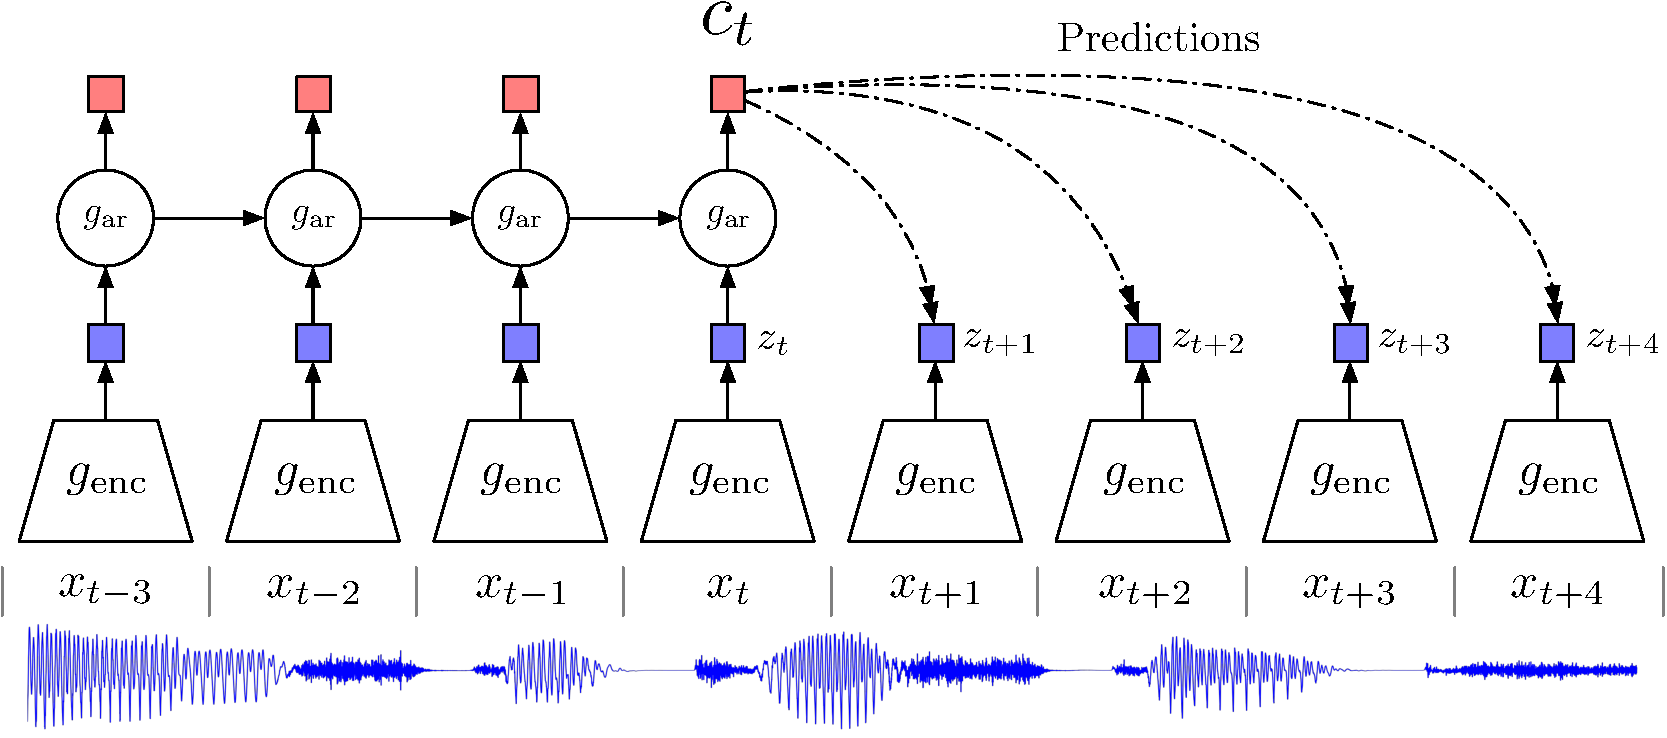
\includegraphics[scale=0.38]{contrastive_repr4.pdf}
    \end{figure}

    \begin{itemize}
      \item \(x_{t_j}\) es la entrada a la red en el instante de tiempo \(t_j\).
      \item \(g_{enc}\) es un codificador que produce una representación \(g_{enc}(x_t) = z_t\)
      \item \(g_{ar}\) es un modelo autorregresivo que produce una representación que tiene en cuenta el contexto \(g_{ar}(z_{\leq t})= c_t\)
    \end{itemize}

      

  
  \end{frame}

  
  \begin{frame}{Pérdida contrastiva y cota inferior contrastiva}
    
    \begin{defi}[Pérdida contrastiva]
      Sea \(X =\{x^*,x_1,\dots,x_{N-1}\}\) un conjunto de \(N\) ejemplos donde $x^*$ ha sido extraido de la distribución conjunta \(P(x,z)\) y le resto han sido extraídos del producto de las distribuciones marginales \(P(x),P(z)\). Se define entonces la función de pérdida contrastiva como  
      \[ 
        \ell(\theta) = - E_X \left[ \log \frac{h_\theta(x^*,z)}{\sum_{x \in X}h_\theta(x,z)}\right]. 
        \]
    \end{defi}

    \begin{prop}
      En las mismas condiciones que en la definición anterior, se tiene que
      \[
        I(x^*,z) \geq -  \ell(\theta) + \log N
      \]
    \end{prop}
  
  \end{frame}
  
  \begin{frame}{Funciones de pérdida usando tripletas}
    \begin{figure}[H]%!htb]
      \minipage{0.32\textwidth}
      \centering
      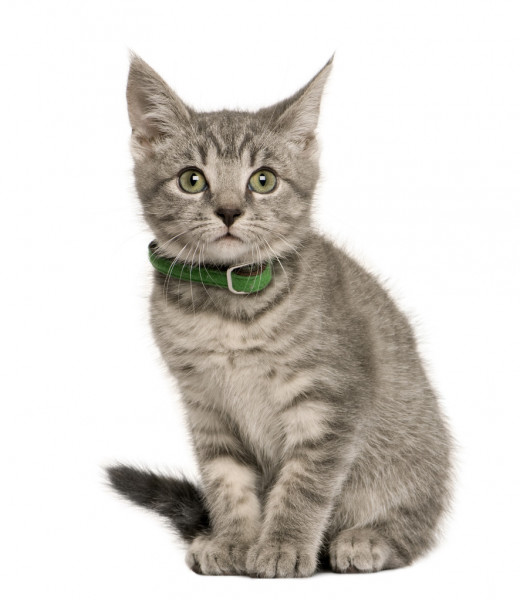
\includegraphics[scale=0.15]{c1}
      \caption*{Original $x$}\label{fig:cat1}
      \endminipage\hfill
      \minipage{0.32\textwidth}%
      \centering
      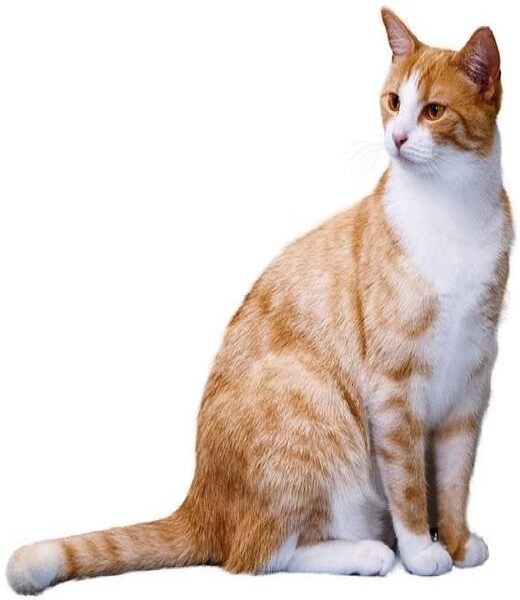
\includegraphics[scale=0.1]{c2}
      \caption*{Ejemplo positivo $\ps$}\label{fig:c2}
      \endminipage
      \minipage{0.32\textwidth}%
      \centering
      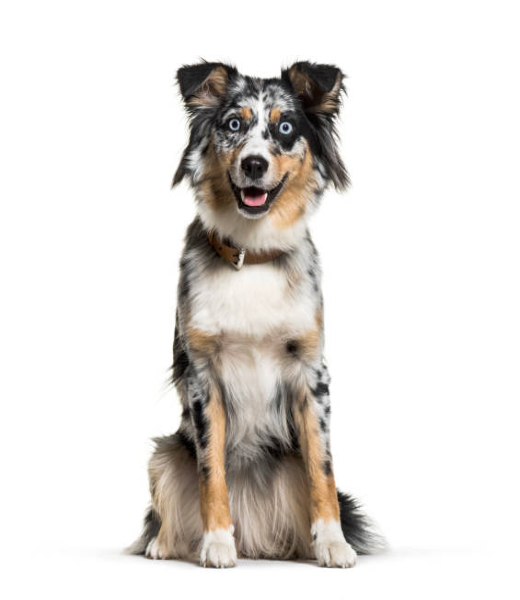
\includegraphics[scale=0.1]{doggo}
      \caption*{Ejemplo negativo $\ns$}\label{fig:doggo}
      \endminipage
    \end{figure}

    \[
    \norm{g(x) - g(\ps)}_2 + \alpha < \norm{g(x) - g(\ns)}_2.
    \]
    \[
      \ell^\alpha (x,\ps,\ns) = \max \left(0, \norm{g(x) - g(\ps)}_2^2 - \norm{g(x) - g(\ns)}_2^2 + \alpha\right).
    \]

  \end{frame}
  
  \begin{frame}{titulo}


    \begin{defi}
      Dado un conjunto de tripletas, cada una con una imagen original, un ejemplo positivo y uno negativo  \(\mathcal T = \{(x_i,\ps_i,\ns_i)\}_{i \in \Lambda} \), una función de pérdida usando tripletas se define como:
      \[
      \mathcal L (x_i,\ps_i,\ns_i) = \sum_{i \in \Lambda} \ell^\alpha(x_i,\ps_i,\ns_i).
      \]

    \end{defi}
    
  
  \end{frame}
  
  \begin{frame}{titulo}
  
  \end{frame}

  
  \begin{frame}{titulo}
  
  \end{frame}
  
  \begin{frame}{titulo}
  
  \end{frame}


\end{document}
